\chapter{Customized PEST setups}
\label{sec:fepest:AdvancedMethods}

PEST is a model independent parameter estimator and as such easy to integrate with most numerical models. The transparent design of its file setup allows the user a lot of customization and to implement own functionality.

One goal in the development of FePEST was to not restrict this flexibility.  It provides a convenient user interface to set up the PEST files, but at any time the user is free to abandon the use of FePEST and continue working with PEST in the traditional way (by direct editing its configuration files and running its tools from the command line).

This release of FePEST implements those PEST features that are commonly used for model calibration. As it was discussed before, PEST has a lot more to offer.

Users that are experienced in using PEST might want to make use of features like Pareto methods or Null-Space Monte-Carlo analysis, or to make changes to certain PEST variables or options that are not accessible through the FePEST GUI. Implementation of own pre- or post-processing code (including third-party software and IFM plug-ins) into the PEST iteration loop might also be desired.

To make the best use of both FePEST and traditional PEST, just configure the PEST setup in FePEST as close as possible to the final settings. Then, generate the respective files, which can be edited as desired. Finally PEST can be started (in some cases, this can be done again from within FePEST).

\section{Creating the PEST setup}

The PEST setup files are created when the PEST run is commenced. To be able to edit the files, press the run button, but disable the options for running PEST (and recalculating the Jacobian if applicable) before pressing the OK button (see Figure \ref{fig:fepest:RunDialogCreateOnly}).


\begin{figure}
	\center
	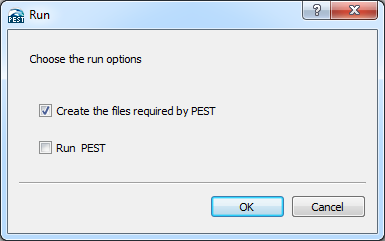
\includegraphics[width=\columnwidth]{figures/RunDialogCreateOnly.png}
\caption{Settings in the Run dialog to create the PEST files.}
\label{fig:fepest:RunDialogCreateOnly}
\end{figure}

The Checks option will also initiate the creation of the files if these are not present when it is executed.

\section{Convenience Tools}

To make the manual editing of the file setup easier, and to allow quick access to the relevant files and locations, the following features become available in the Estimation menu of FePEST after the PEST files have been generated.

\begin{itemize}
\item Checks

Runs the PEST error check tools PESTCHEK (checks the control file), INSCHECK (checks the instructions file) and TEMPCHEK (checks the template file). Errors and warnings - if raised - will be shown in the dialog. 

\item Open work folder in explorer

Use this option to open the work folder, operate with files or to open them for editing.

\item Open work folder in console window

Use this option to open a new command line window, from where PEST (and other) commands can run.

\item Open control file

Directly opens the PEST control (pst) file in the standard editor.

\item Show command

Shows a command line string with that the PEST run can be initiated. Use this command if you want to run PEST outside the FePEST GUI.
\end{itemize}

\section{File Structure}

Figure \ref{fig:fepest:FileStructure} shows the basic file structure as it is created by FePEST for the simplest case. Additional files may be present depending on the selected methods.

\begin{itemize} 
\item PEST script (run\_pest.bat)

This script file is executed when the PEST run is started by the user within FePEST. Besides other commands, the PEST executable is called. The content of this script will vary depending on the settings done in FePEST (e.g., SVDAPREP will be run from this script if SVD-Assist is active).

Change this script to implement additional commands to the overall PEST process.

\item Model script (run\_model.bat)

This script is executed by PEST directly to commence a model call (It is cited as the model command in the PEST control file). The actual FEFLOW execution is cited in here.

Attention: This file is automatically re-generated when the PEST run commences, to allow cross-computer and cross-platform compatibility during parallel BeoPEST runs. To effectively change this file, create a copy and update the command line in the PEST control accordingly.

Add commands to this file that should be executed with every model run.

\item FePEST input file (\textless  case\textgreater.fpi)	

PEST writes parameter values to the FePEST input file (as advised in the respective template file), from where they are read by FePEST. The format is kept very simple, thus that user-specific scripts or plug-ins can access it. 

In case at least one IFM-implemented observation is present, a second input file (ifm.in) is created. IFM-implemented observations appear in this file. The observation value will be set to the default value when the model is called, to allow a successful PEST run in case the observation is not handled.

\item FePEST output file (\textless  case\textgreater.fpo)

FePEST writes observation values to the FePEST output file, from where they are read by PEST (as advised in the respective instructions file). Once again, a very simple format is used thus that user-defined scripts or plug-ins can access this file.

In case at least one IFM-implemented parameter is present, a second output file (ifm.out) is created. IFM-implemented parameters appear in this file.

\item PEST control file (\textless  case\textgreater.pst)
 
This is the primary PEST control file which defines the configuration of PEST. Edit this file to make changes that are not supported by FePEST.

\item SVDA files (super.pst and others)

If SVD-Assist is used, a second pest setup will appear in the directory after SVDAPREP has been executed by the PEST script.  

\item Supportive files

Other files may appear depending on settings. E.g., several PLPROC files will be generated if the pilot-point method is applied, and a covariance matrix will be created by PPCOV if pilot-points are regularized.

\end{itemize}

\textit{The FePEST help contains a detailed description of these and other files.}

\begin{figure*}
	\center
	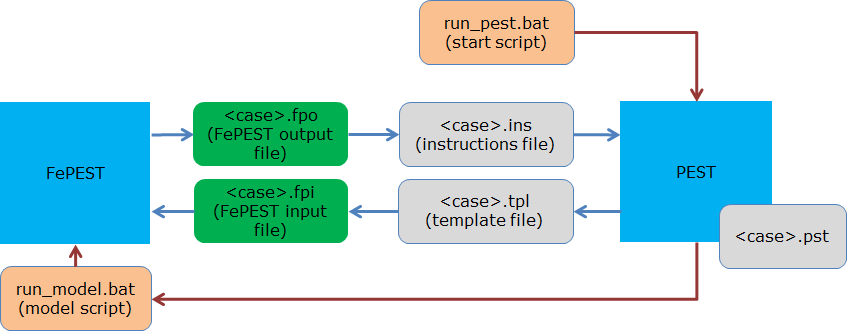
\includegraphics[width=2\columnwidth]{figures/FileStructure.png}
\caption{PEST file structure created by FePEST. Additional files may be present depending on the used methods (e.g., SVDA or pilot points)}
\label{fig:fepest:FileStructure}
\end{figure*}

\section{Running Customized PEST Setups}

A customized setup of files can be run in two ways: Either from within or outside of FePEST:

\begin{itemize}
\item Run from within FePEST

This option is more convenient and should be preferred if applicable. Click on Run again, but deactivate the Create Files option this time (otherwise, the files would be overwritten, see Figure \ref{fig:fepest:RunDialogRunOnly}).

\begin{figure}
	\center
	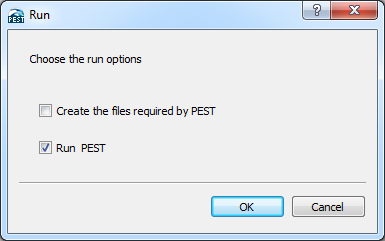
\includegraphics[width=\columnwidth]{figures/RunDialogRunOnly.png}
\caption{Settings in the Run dialog to run PEST without recreating the file setup.}
\label{fig:fepest:RunDialogRunOnly}
\end{figure}

FePEST will commence the PEST run by running the PEST script (run\_pest.bat under windows), including all user modifications.

Note that because FePEST parses the primary output of PEST during run-time, FePEST visual feedback might fail partially or completely if the PEST output changes significantly due to the user modifications.

\item PEST script from command line

The FePEST is part of a superordinate batch run, the PEST script (or its contents) can be incorporated into another script.

Even though visual feedback cannot be provided any more, FePEST (called in its simulation mode) still ensures that parameters and observations are correctly transferred between FEFLOW and PEST.
\end{itemize}

\section{Integration of IFM Plug-ins and Third-Party Code}

When creating a new observation definition or parameter definition, FePEST offers the type "IFM implemented" to add a specified numbers of additional parameters to the PEST file setup. These can be directly modified by an IFM plug-In or a third-party code (e.g., a script or another program).

\begin{itemize}
\item IFM plug-ins

An IFM plug-in must be attached to the FEFLOW model and registered in FEFLOW before the PEST run is started. If parallelization is used that involves remote servers, the plug-in must be installed on all remote machines as well (plug-ins will not be transferred automatically).

The plug-in can than open the fpi-file during run-time of the model to read parameters, and opens the fpo-file to save observations.

\item Scripts and third-party software

Any program used for additional postprocessing can access the fpi (to read parameters) and fpo file (to save observations) accordingly. To include them in the optimization, they have to be started appropriately from one of the batch files (either the model batch file or the pest run batch file).

For user-defined parameters, consider creating a new parameter group with appropriate settings for the derivative calculation.

\end{itemize}